\section{Background}
\label{sec:bg}

In this section, we provide relevant details pertaining to the NEMD simulation in~\ref{sub:nemd}, and
key theoretical aspects of the active subspace methodology in~\ref{sub:as}.

\subsection{NEMD simulation}
\label{sub:nemd}

The NEMD simulations in this work were performed using the LAMMPS software package~\cite{Plimpton:2007}.
Specifically, the simulations were performed for a Si bar of length, $L$, subjected to a temperature gradient, 
$\left(\frac{dT}{dz}\right)$. The temperature gradient was applied by means of Langevin thermostats located
at $L/4$ and $3L/4$. Schematic illustration of the set-up and the arrangement of atoms is provided below in 
Figure~\ref{fig:setup}.

\begin{figure}[htbp]
\begin{center}
\begin{tabular}{cc}
  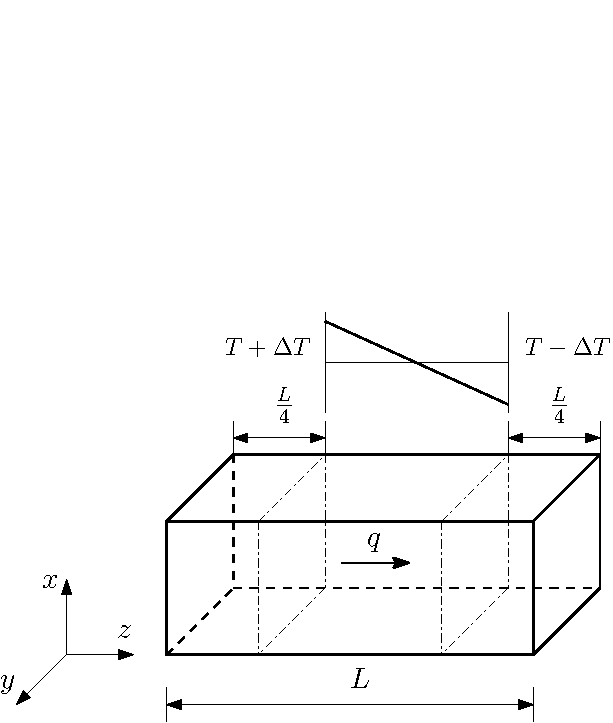
\includegraphics[width=0.48\textwidth]{./Figures/schematic}
  &
  \hspace{3mm}
  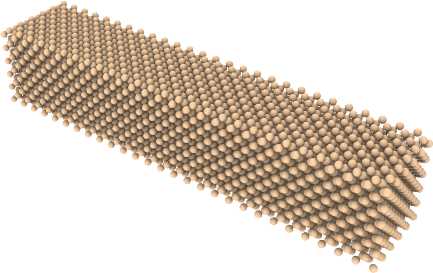
\includegraphics[width=0.40\textwidth]{./Figures/Sibar_05}
  \\ (a) & (b)
  \end{tabular}
\caption{(a) Schematic illustration of the simulation set-up for estimating the thermal conductivity of a Si bar of
length, $L$, subjected to a temperature gradient, $\left(\frac{4\Delta T}{L}\right)$, (b) 
Initial configuration of Si atoms in the bar.}
\label{fig:setup}
\end{center}
\end{figure}
%
The heat flux between the thermostats at the end of the simulation ($q$, W/m$^2$) is recorded to compute the
thermal conductivity of the Si bar using Fourier's law:
%
\be
 \kappa = \frac{q}{\left|\frac{dT}{dz}\right|} 
\ee
%
where $\left|\frac{dT}{dz}\right|$ denotes the magnitude of the applied thermal gradient. In table~\ref{tab:input},
we provide the set of inputs used to perform the NEMD simulation. Note that the simulation run length, width, 
and height were selected to minimize temperature fluctuations during the different stages of the simulation while
ensuring a reasonable computational effort. 
%
\begin{table}[htbp]
\centering
\ra{1.3}
\begin{tabular}{@{}cc@{}}\toprule
Lattice Constant, $a$ ($\angstrom$) & 5.43 \\ 
Width, Height ($\angstrom$) & 22$a$ \\
$\Delta t$  (ps) & 0.0005 \\ 
Simulation Run Length (ps) & 320 \\ 
Boundary Condition & Periodic \\ 
Lattice Structure & Diamond \\
Inter-atomic Potential & Stillinger-Weber \\ 
\bottomrule
\end{tabular}
\caption{The set of LAMMPS inputs for performing the NEMD simulation of a Si bar illustrated in Figure~\ref{fig:setup}.}
\label{tab:input}
\end{table}
 
As illustrated in the following flow diagram, there are three stages involved in the NEMD simulation: NVT, NVE (I), and
NVE (II); NVT and NVE are thermodynamic ensembles used commonly in NEMD simulations. We have used
(I) and (II) here to distinguish between the two NVE ensembles. 
%
\begin{center}
NVT \hspace{5mm} $\rightarrow$ \hspace{5mm} NVE (I) \hspace{5mm}
$\rightarrow$ \hspace{5mm} NVE (II)
\\ \vspace{1mm}
\tiny \hspace{-5mm}[Equilibrate system to 300 K] \hspace{1mm} [Equilibrate thermostats] \hspace{4mm}
 [Generate Data]
\\ \vspace{1mm}
\tiny{N: Number of Atoms~~~V: Volume~~~T: Temperature~~~E: Energy}
\end{center}
%
During the NVT stage, the system is equilibrated to a specific bulk temperature at which the thermal conductivity
of the bar is to be estimated. The NVE (I) stage involves equilibration of the thermostats at specified temperatures.
Lastly, during the NVE (II) stage, the trajectory of individual atoms during simulation is recorded.

\subsection{Active Subspace}
\label{sub:as}
